\section{RENCANA DESAIN UI/UX}

\subsection{Pendekatan User Research yang Akan Dilakukan}

Untuk memahami kebutuhan pengguna sebelum mulai implementasi, akan dilakukan penelitian sebagai berikut:

\begin{enumerate}[leftmargin=*]
    \item \textbf{Wawancara dengan UMKM Kuliner} : Akan dilakukan wawancara mendalam untuk memahami tantangan mereka dalam pengelolaan makanan surplus.
    
    \item \textbf{Survei Online} : Akan disebarkan kuesioner kepada konsumen potensial untuk mengetahui preferensi pembelian makanan surplus.
    
    \item \textbf{Observasi Lapangan} : Akan dilakukan pengamatan langsung terhadap operasional UMKM kuliner untuk mengidentifikasi pain points.
\end{enumerate}

\textbf{CATATAN}: Research ini akan dilakukan pada fase awal development, belum dilaksanakan saat ini.

\subsection{Target User Persona (Draft)}

\subsubsection{Persona 1: UMKM Kuliner (Draft)}
\begin{table}[htbp]
\centering
\begin{tabularx}{0.8\textwidth}{|l|X|}
\hline
\textbf{Aspek} & \textbf{Karakteristik} \\
\hline
Usia & 30-55 tahun \\
\hline
Usaha & Warung makan, kafe, katering \\
\hline
Teknologi & Cukup mahir menggunakan smartphone \\
\hline
Kebutuhan & Mengurangi food waste, menambah pendapatan \\
\hline
Pain Point & Kesulitan prediksi permintaan, tidak ada platform khusus \\
\hline
\end{tabularx}
\end{table}

\subsubsection{Persona 2: Customer (Draft)}
\begin{table}[htbp]
\centering
\begin{tabularx}{0.8\textwidth}{|l|X|}
\hline
\textbf{Aspek} & \textbf{Karakteristik} \\
\hline
Usia & 18-40 tahun (milenial dan Gen Z) \\
\hline
Pekerjaan & Mahasiswa, karyawan swasta \\
\hline
Kebutuhan & Makanan berkualitas dengan harga terjangkau \\
\hline
Pain Point & Ketidakyakinan terhadap kelayakan makanan diskon \\
\hline
\end{tabularx}
\end{table}

\subsubsection{Persona 3: Admin Platform (Draft)}
\begin{table}[htbp]
\centering
\begin{tabularx}{0.8\textwidth}{|l|X|}
\hline
\textbf{Aspek} & \textbf{Karakteristik} \\
\hline
Usia & 25-45 tahun \\
\hline
Peran & Operator platform, moderator \\
\hline
Kebutuhan & Monitoring transaksi, verifikasi UMKM \& Mitra Donasi, keuangan platform \\
\hline
\end{tabularx}
\end{table}

\subsubsection{Persona 4: Mitra Donasi (Draft)}
\begin{table}[htbp]
\centering
\begin{tabularx}{0.8\textwidth}{|l|X|}
\hline
\textbf{Aspek} & \textbf{Karakteristik} \\
\hline
Bentuk & Yayasan, panti, komunitas sosial, bank makanan \\
\hline
Peran & Menerima makanan surplus dari UMKM \\
\hline
Kebutuhan & Registrasi mudah, verifikasi legalitas, akses makanan surplus \\
\hline
Pain Point & Sulit menemukan sumber donasi makanan yang rutin dan tepercaya \\
\hline
\end{tabularx}
\end{table}

\subsection{Antarmuka Aplikasi (Prototipe)}

Prototipe antarmuka Savora telah dibangun dengan Next.js dan Tailwind CSS mengikuti prinsip
\textit{mobile-first} serta heuristik usability Nielsen \cite{nielsen2020heuristics}. Berikut
tangkapan layar dari halaman-halaman utama. Layar untuk alur \textit{cashless} (checkout Midtrans,
\textit{pickup code}), Help Center, Waste Log, serta registrasi/verifikasi Mitra Donasi merupakan
bagian MVP yang sedang diselesaikan dan dirangkum pada inventaris layar (Tabel~\ref{tab:screens}).

\subsubsection{Alur Customer}

\begin{figure}[htbp]
\centering
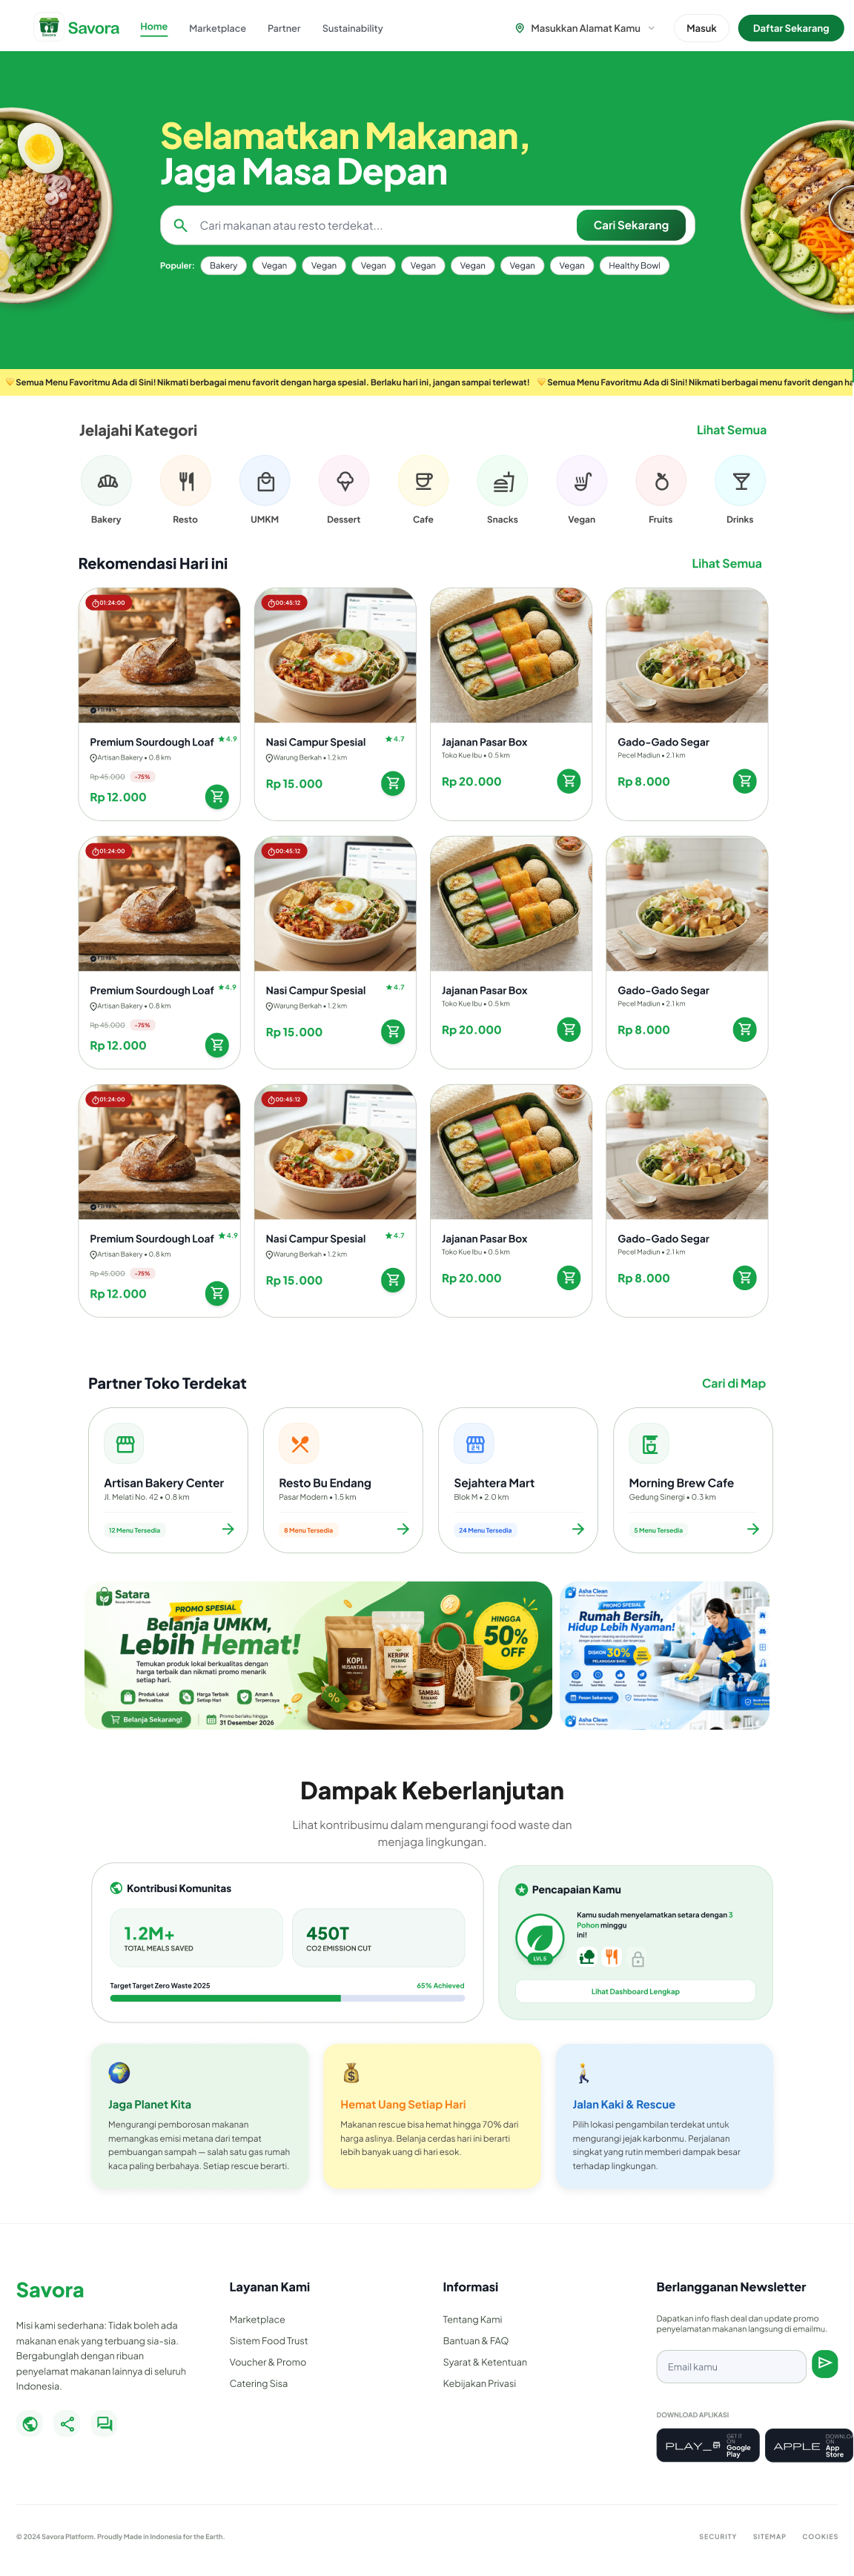
\includegraphics[width=0.74\textwidth, height=6.6cm, keepaspectratio]{gambar/beranda-customer.png}
\caption{Beranda / Marketplace Customer dengan Food Score dan timer rescue}
\label{fig:ui_beranda}
\end{figure}

\subsubsection{Alur UMKM}

% Dua dashboard UMKM disandingkan agar padat dan tidak menyisakan ruang kosong
\begin{figure}[htbp]
\centering
\begin{minipage}[t]{0.49\textwidth}
\centering
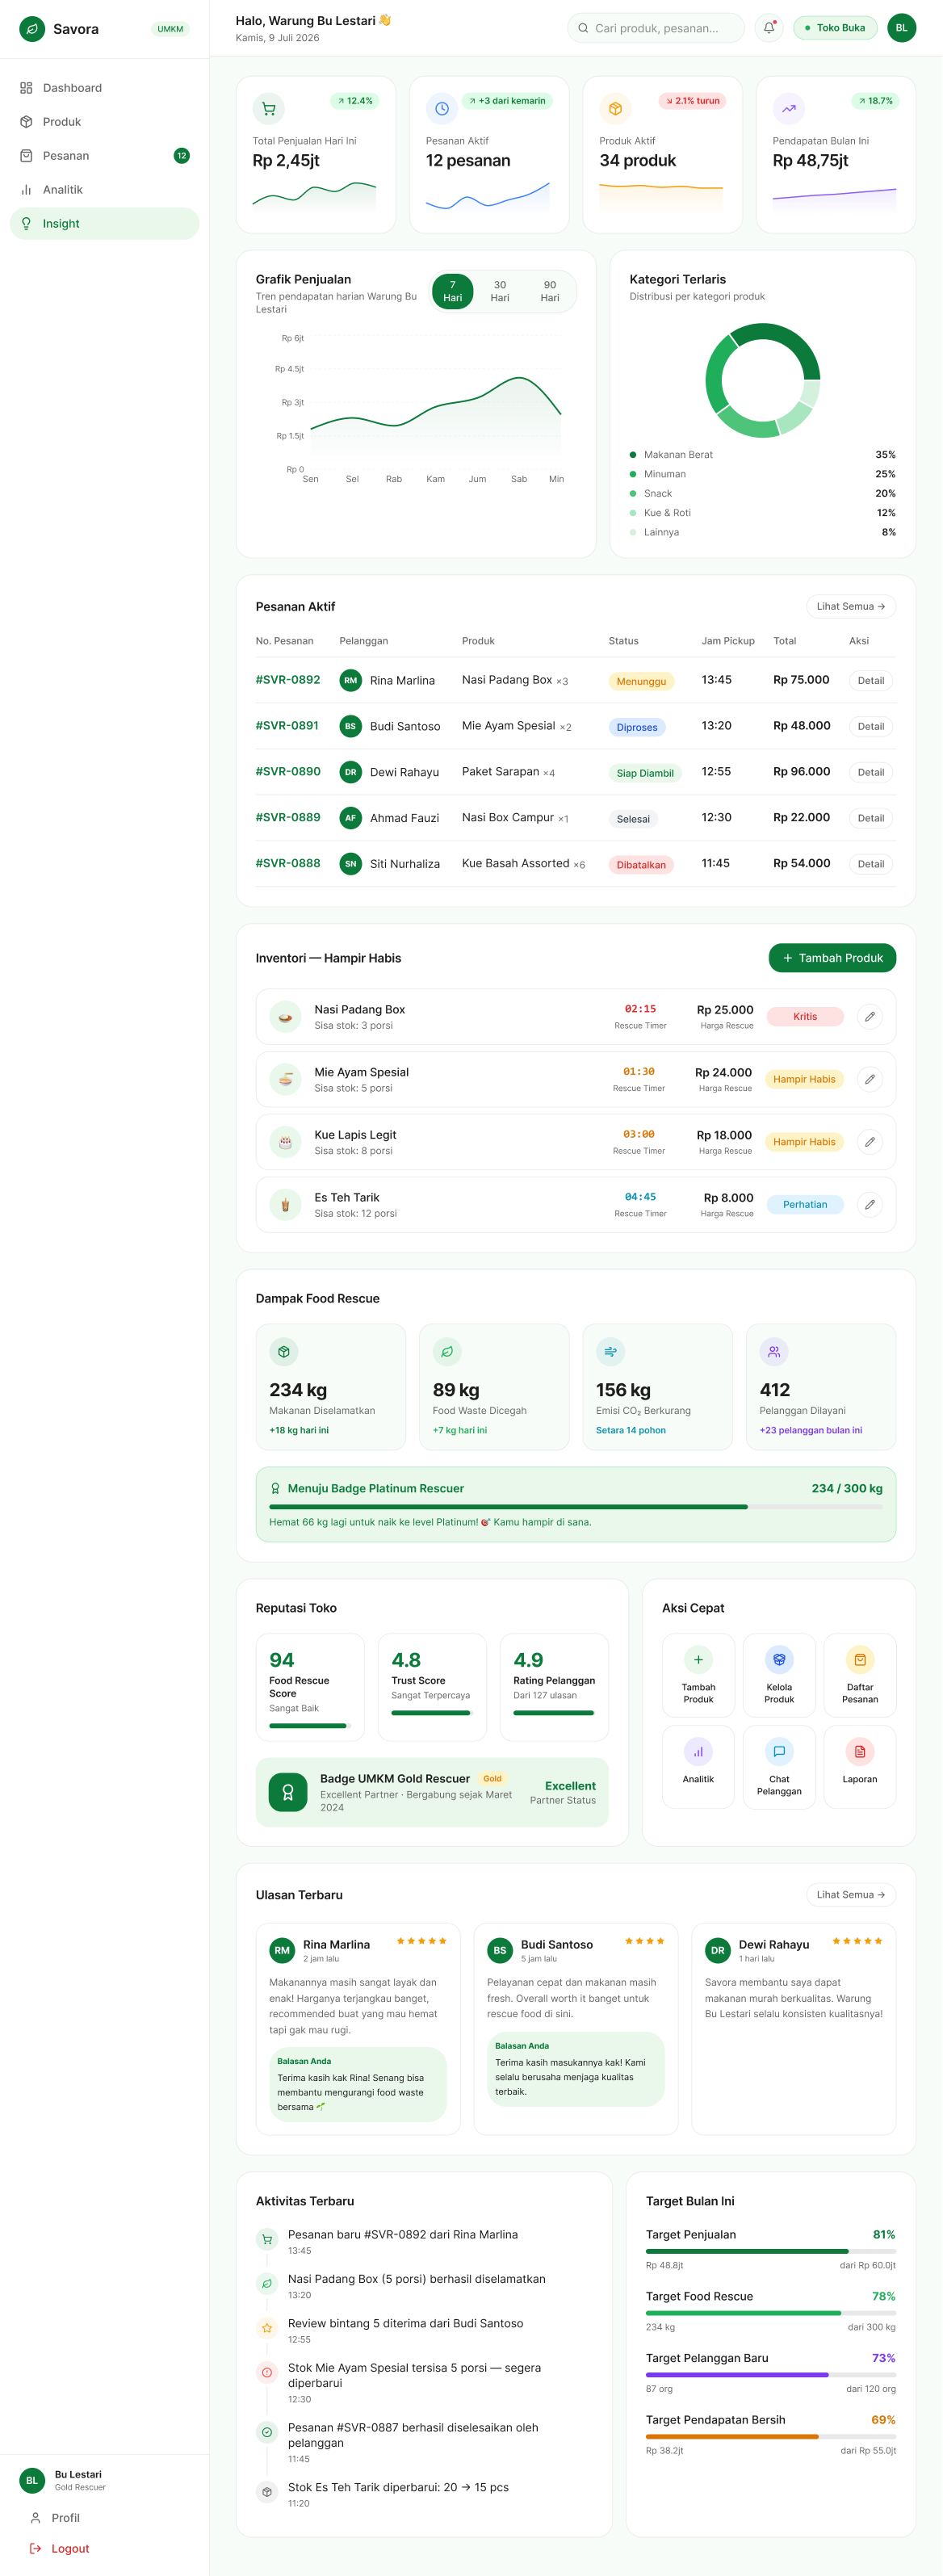
\includegraphics[width=\linewidth, height=5.2cm, keepaspectratio]{gambar/dashboard-umkm.png}
\caption{Dashboard UMKM}
\label{fig:ui_dashboard}
\end{minipage}\hfill
\begin{minipage}[t]{0.49\textwidth}
\centering
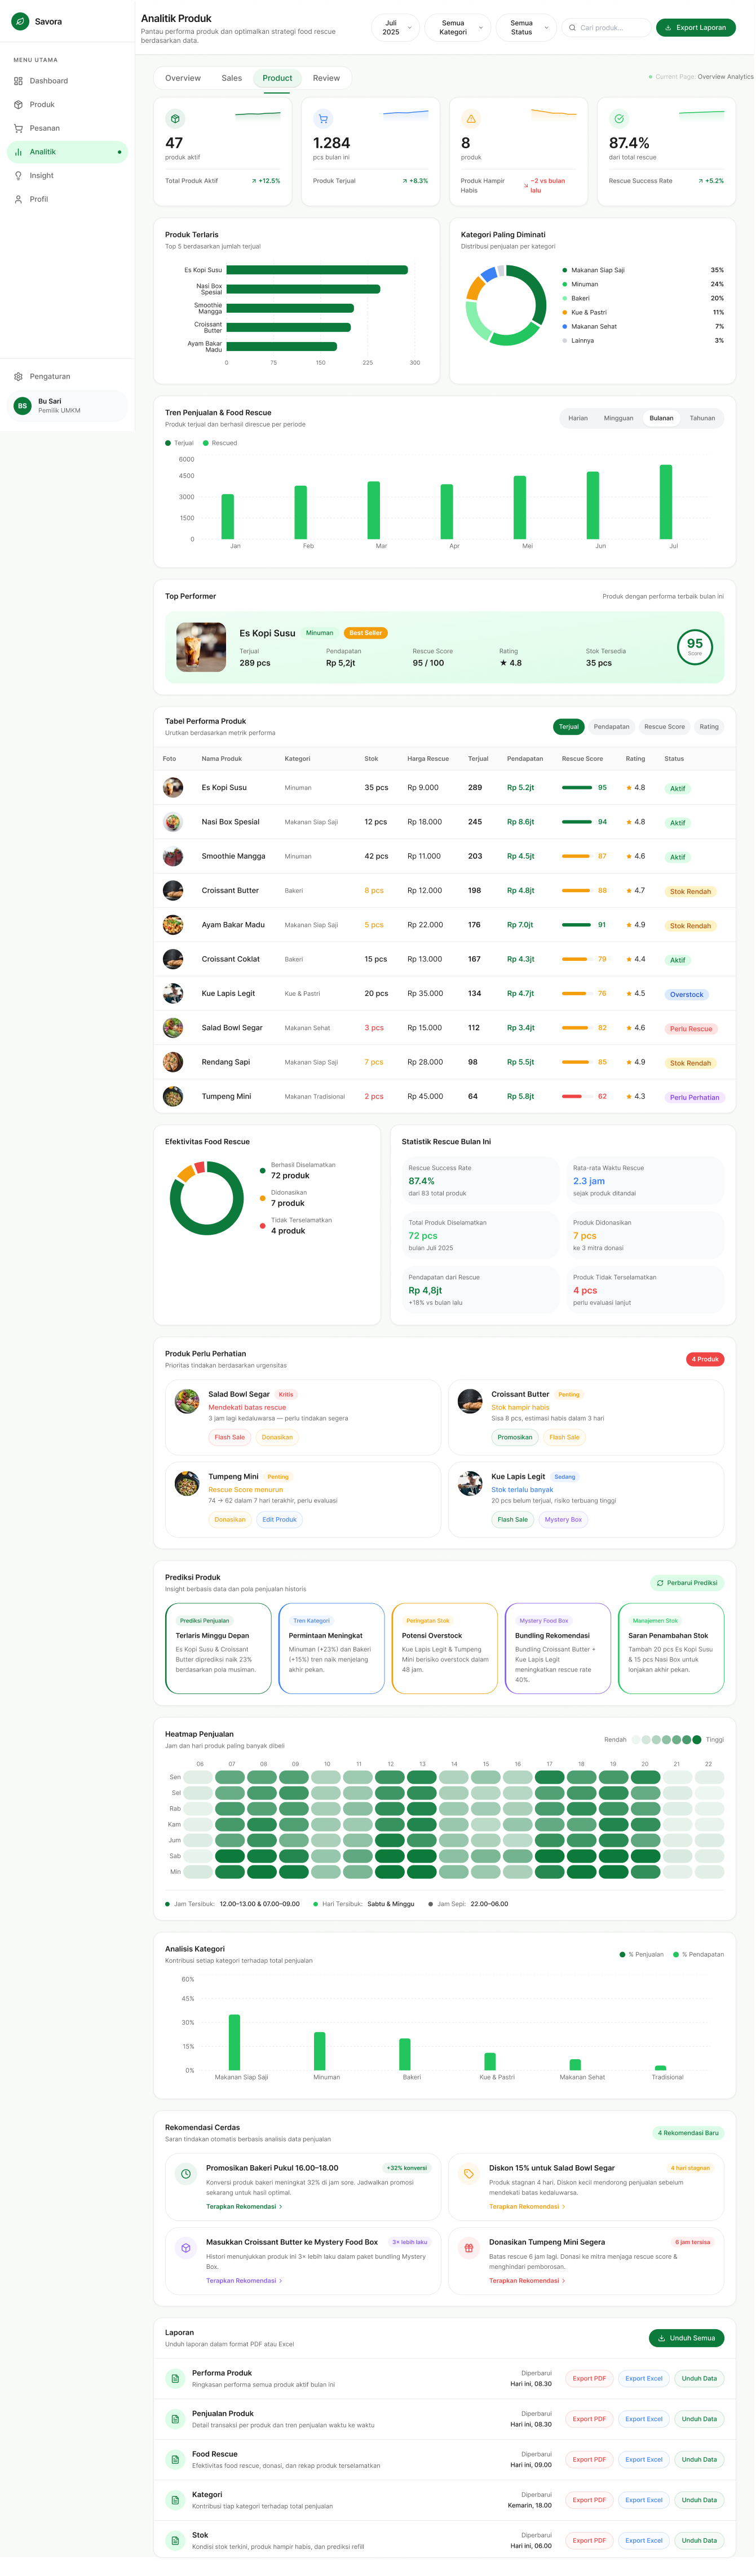
\includegraphics[width=\linewidth, height=5.2cm, keepaspectratio]{gambar/analitik-produk.png}
\caption{Analitik Produk UMKM}
\label{fig:ui_analitik}
\end{minipage}
\end{figure}

\begin{figure}[htbp]
\centering
\begin{minipage}[t]{0.49\textwidth}
\centering
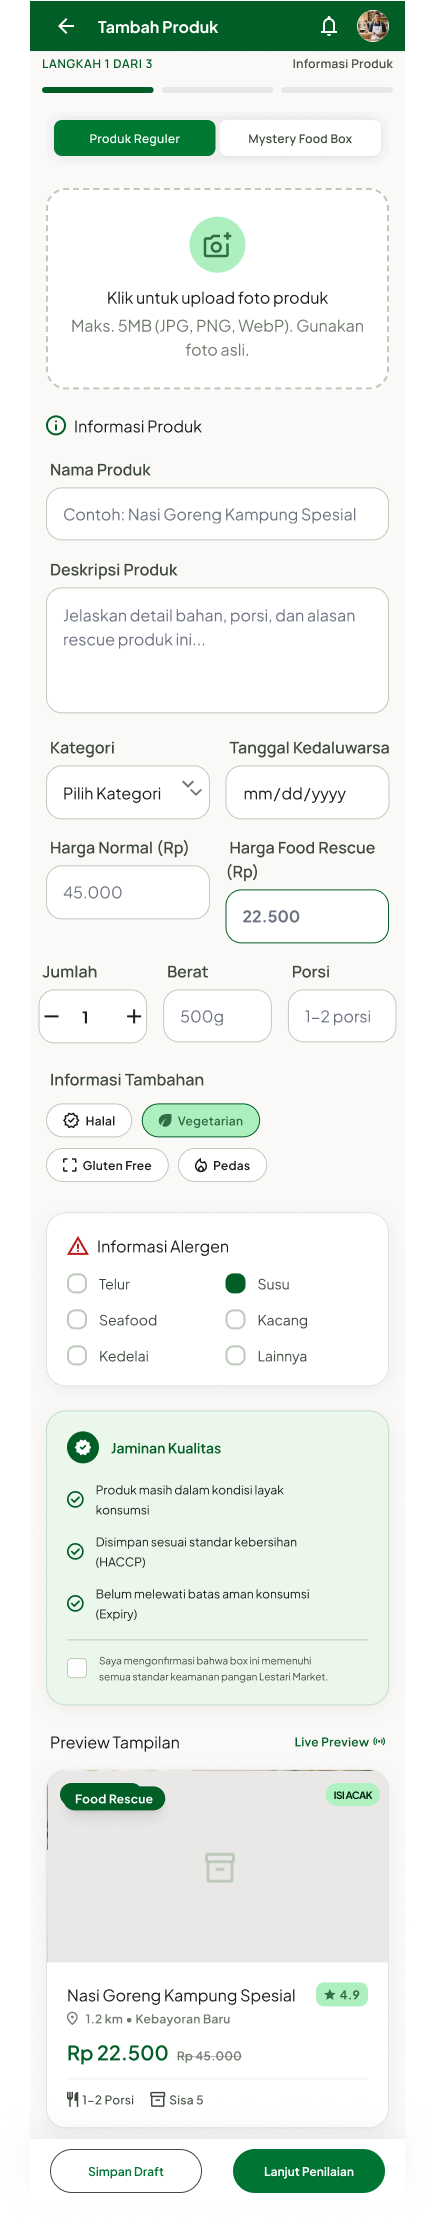
\includegraphics[width=\linewidth, height=6.4cm, keepaspectratio]{gambar/tambah-produk-reguler.png}
\caption{Tambah Produk Reguler}
\label{fig:ui_produk_reguler}
\end{minipage}\hfill
\begin{minipage}[t]{0.49\textwidth}
\centering
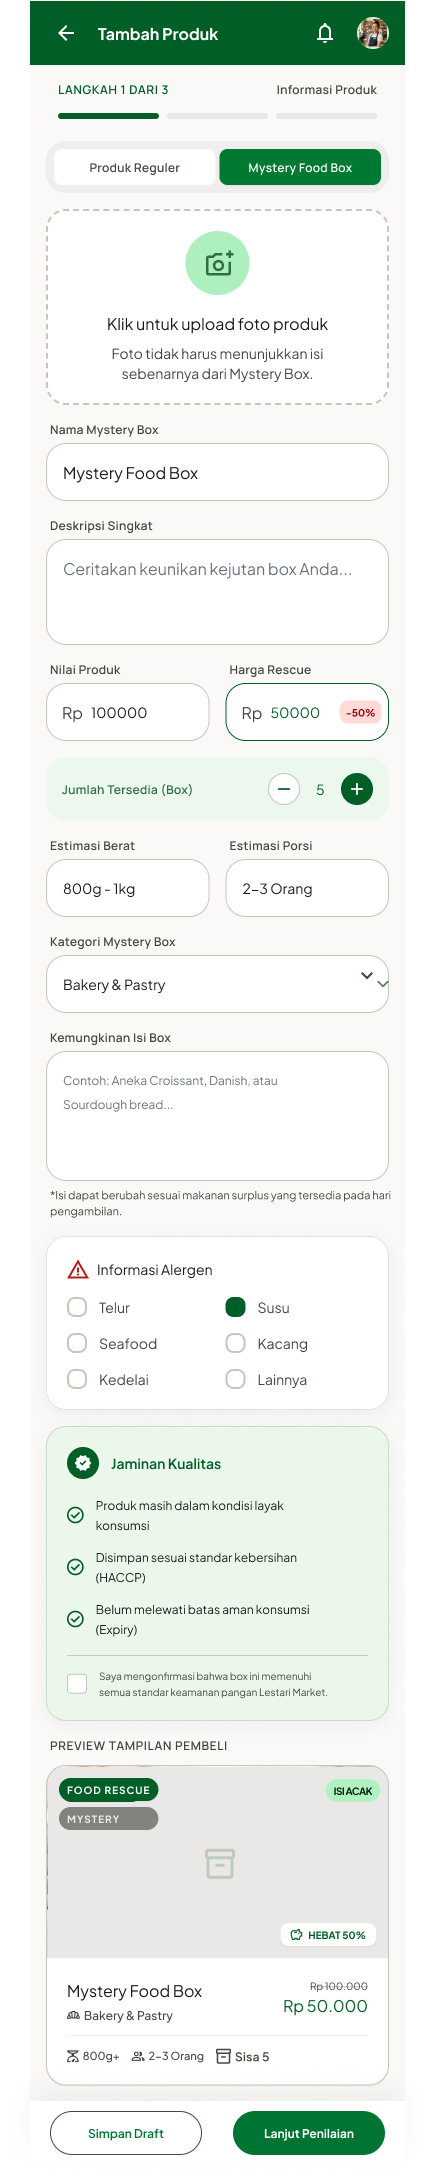
\includegraphics[width=\linewidth, height=6.4cm, keepaspectratio]{gambar/tambah-produk-mysterybox.png}
\caption{Tambah Produk Mystery Box}
\label{fig:ui_produk_mb}
\end{minipage}
\end{figure}

\begin{figure}[htbp]
\centering
\begin{minipage}[t]{0.49\textwidth}
\centering
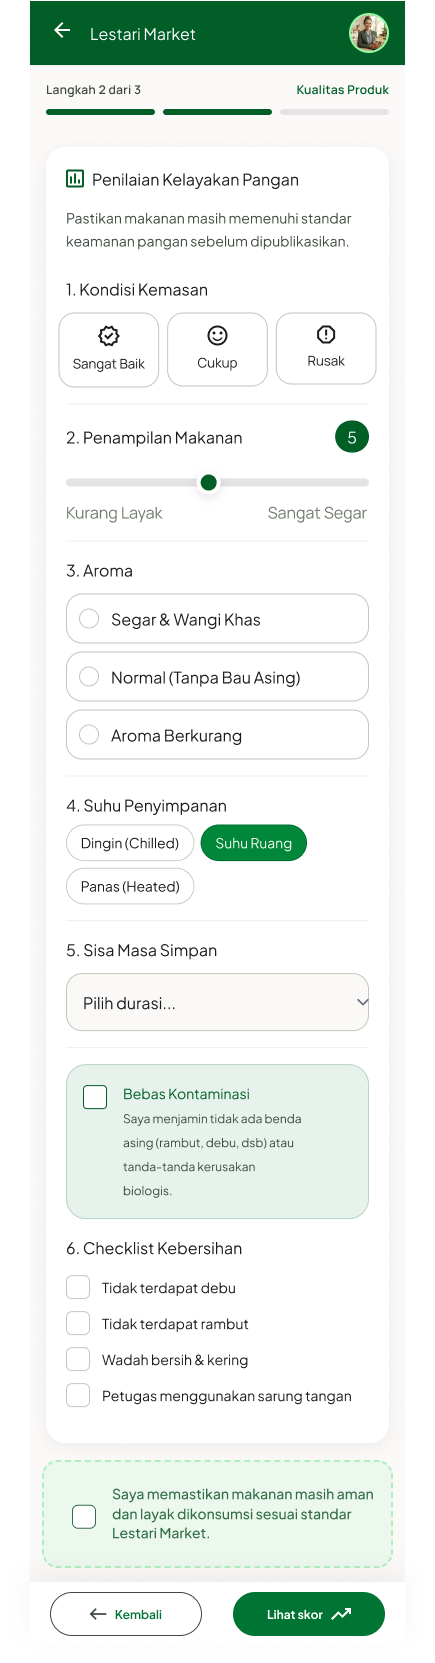
\includegraphics[width=\linewidth, height=6.4cm, keepaspectratio]{gambar/penilaian-kelayakan.png}
\caption{Form Penilaian Kelayakan}
\label{fig:ui_penilaian}
\end{minipage}\hfill
\begin{minipage}[t]{0.49\textwidth}
\centering
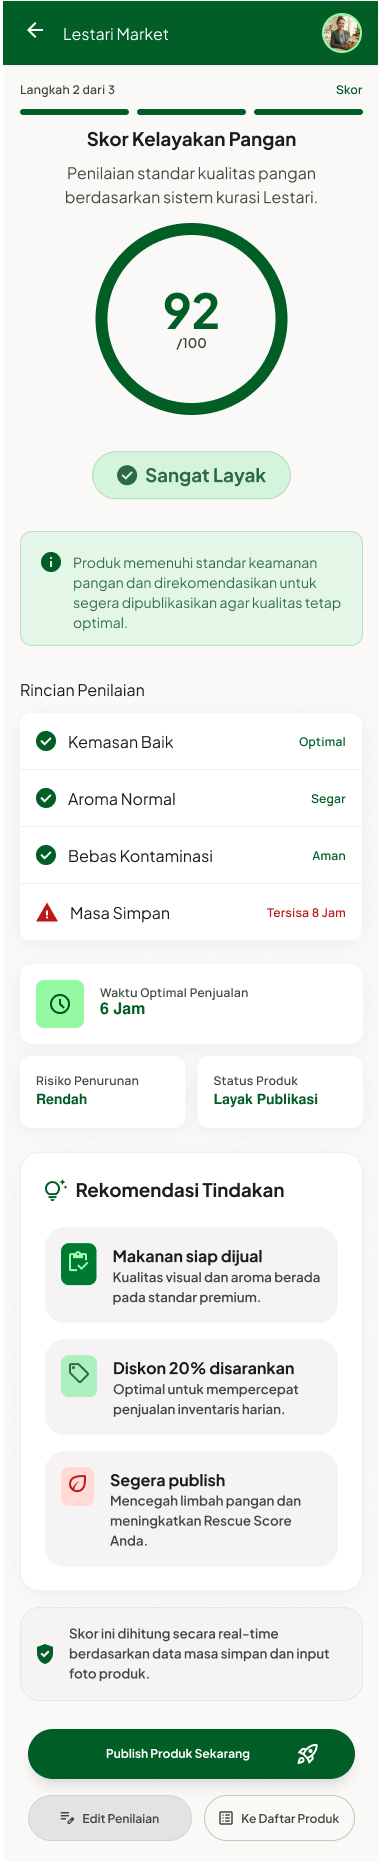
\includegraphics[width=\linewidth, height=6.4cm, keepaspectratio]{gambar/hasil-kelayakan.png}
\caption{Hasil Food Trust Index}
\label{fig:ui_hasil}
\end{minipage}
\end{figure}

\subsubsection{Alur Autentikasi dan Admin (Direncanakan)}

\begin{figure}[htbp]
\centering
\begin{minipage}[t]{0.49\textwidth}
\centering
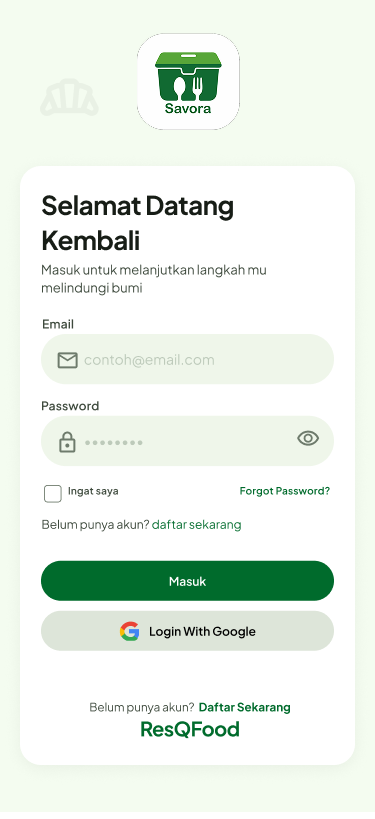
\includegraphics[width=\linewidth, height=6.0cm, keepaspectratio]{gambar/login.png}
\caption{Halaman Login}
\label{fig:ui_login}
\end{minipage}\hfill
\begin{minipage}[t]{0.49\textwidth}
\centering
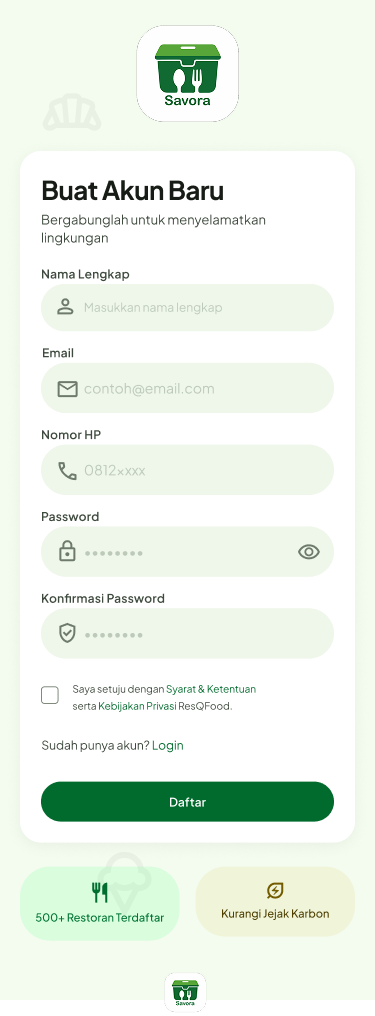
\includegraphics[width=\linewidth, height=6.0cm, keepaspectratio]{gambar/register.png}
\caption{Halaman Register}
\label{fig:ui_register}
\end{minipage}
\end{figure}

\begin{figure}[htbp]
\centering
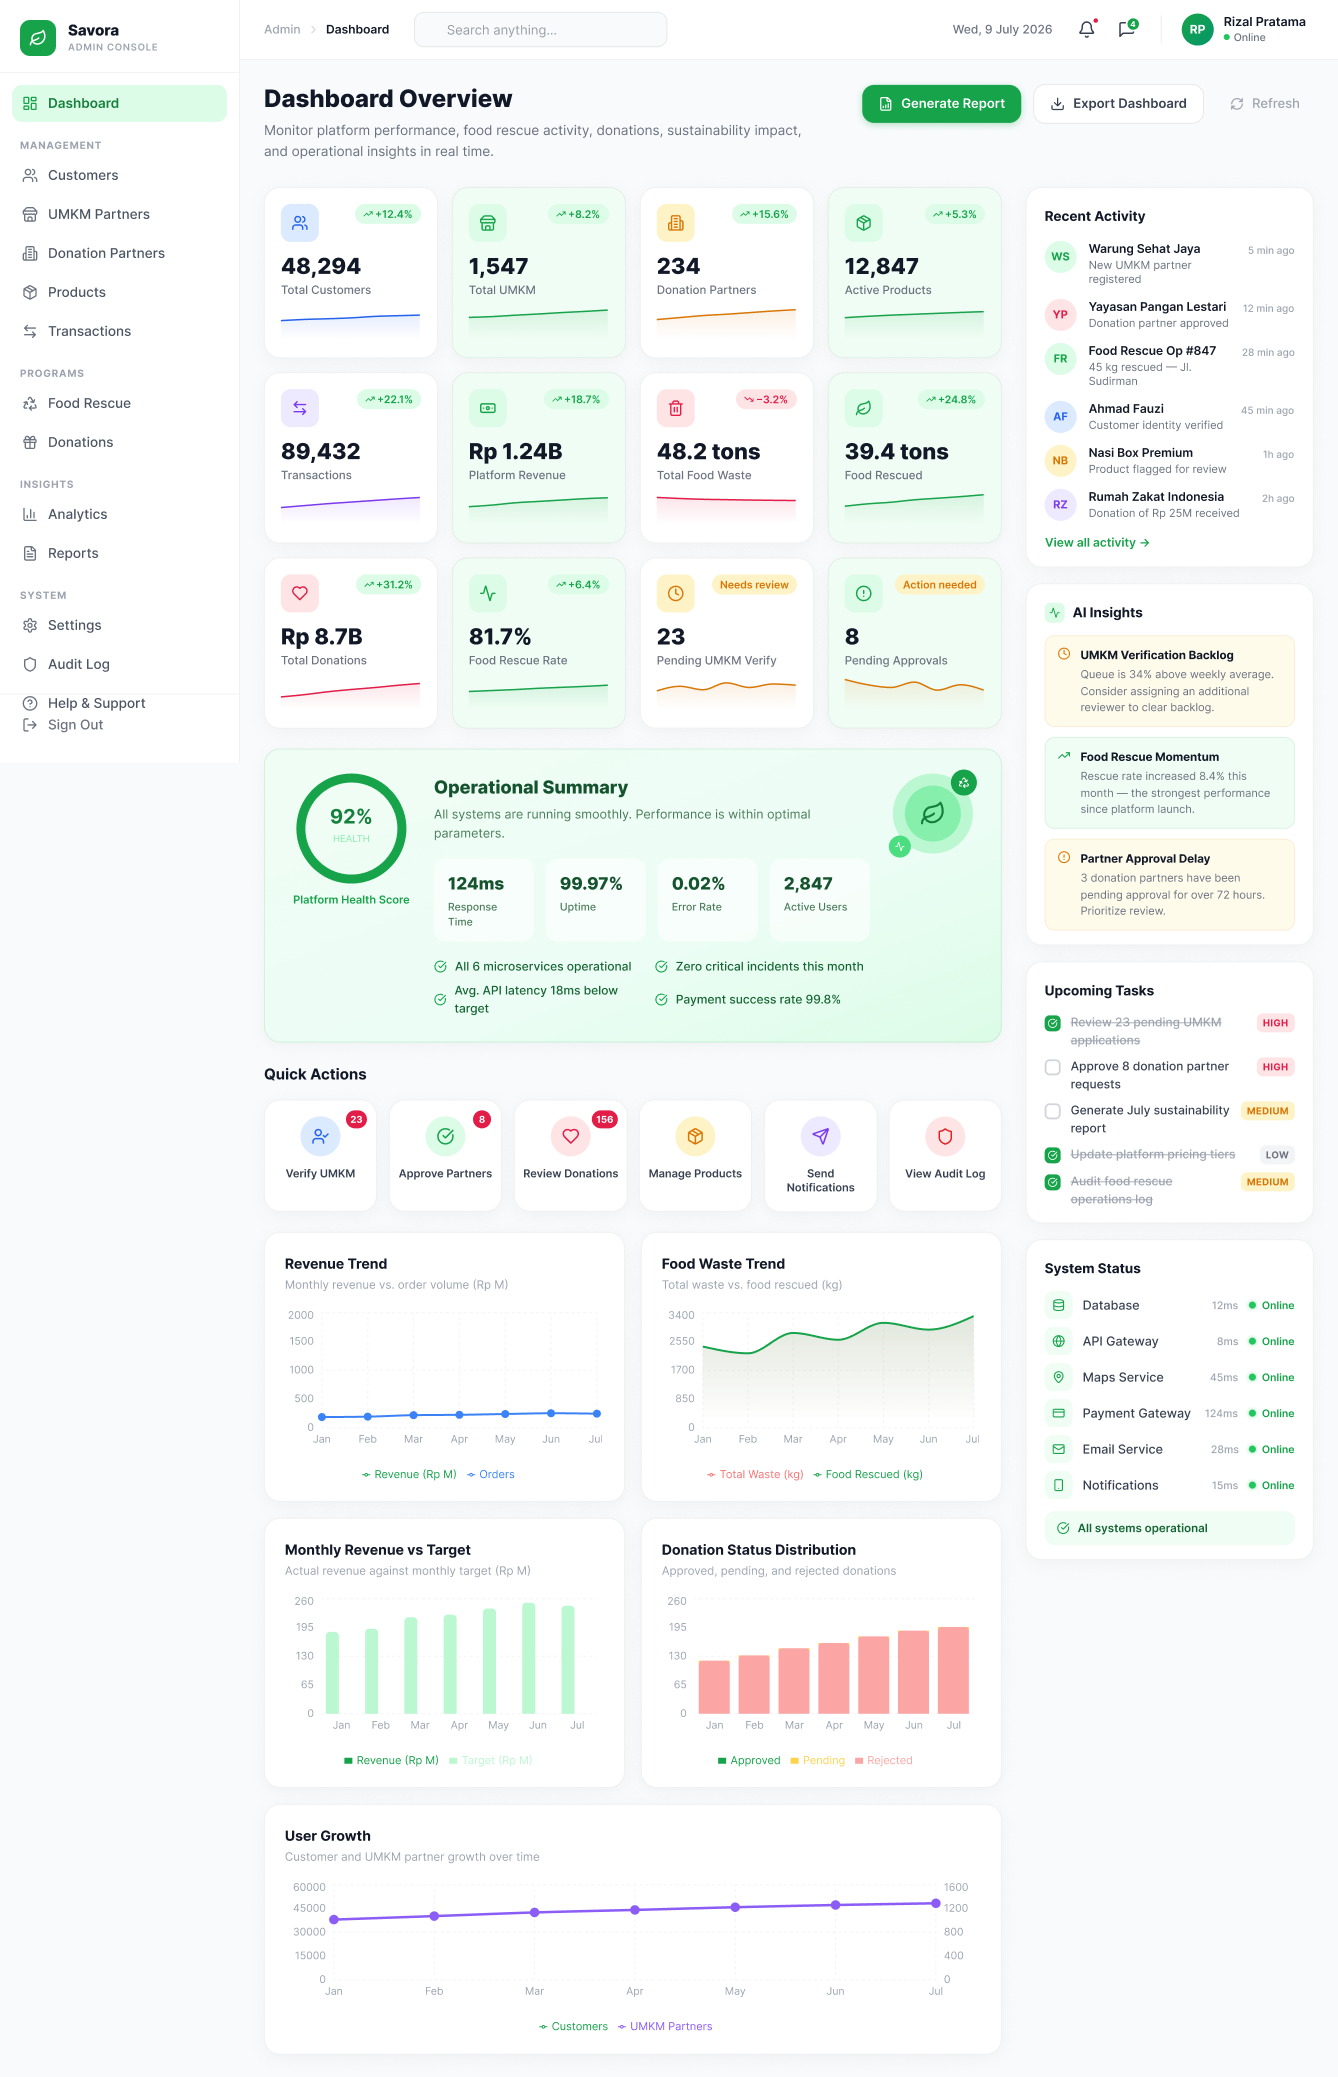
\includegraphics[width=0.74\textwidth, height=6.6cm, keepaspectratio]{gambar/admin-console.png}
\caption{Admin Console (direncanakan)}
\label{fig:ui_admin}
\end{figure}

\subsection{Inventaris Layar MVP}

Tabel~\ref{tab:screens} merangkum layar utama pada rancangan MVP beserta statusnya, agar cakupan
UI selaras dengan ruang lingkup fungsional.

\begin{table}[htbp]
\centering
\caption{Inventaris Layar MVP Savora}
\label{tab:screens}
\small
\begin{tabularx}{\textwidth}{|l|X|l|}
\hline
\textbf{Aktor} & \textbf{Layar} & \textbf{Status} \\
\hline
Customer & Marketplace (Food Score, timer, badge keyword) & Sudah berjalan \\
\cline{2-3}
& Detail produk \& detail UMKM & Sudah berjalan \\
\cline{2-3}
& Checkout cashless + service fee, status \& pickup code & Direncanakan \\
\cline{2-3}
& Help Center (buat tiket) & Direncanakan \\
\hline
UMKM & Dashboard, analitik, insight & Sudah berjalan \\
\cline{2-3}
& Tambah produk (reguler \& mystery box) & Sudah berjalan \\
\cline{2-3}
& Form Food Trust Index \& hasil kelayakan & Sudah berjalan \\
\cline{2-3}
& Validasi pickup code \& Waste Log & Direncanakan \\
\hline
Admin & Verifikasi UMKM \& Mitra Donasi, moderasi & Direncanakan \\
\cline{2-3}
& Dashboard keuangan \& export laporan & Direncanakan \\
\hline
Mitra Donasi & Registrasi \& status verifikasi & Direncanakan \\
\hline
Umum & Login / Register (4 role) & Direncanakan \\
\hline
\end{tabularx}
\end{table}

\subsection{Aksesibilitas dan Prinsip Desain}

Antarmuka Savora dirancang mengikuti prinsip aksesibilitas praktis agar dapat digunakan oleh
rentang pengguna yang luas:

\begin{itemize}[leftmargin=*]
    \item \textbf{Kontras warna} : Status Food Score/rescue timer tidak hanya dibedakan warna
    (merah/kuning/hijau) tetapi juga label teks, agar tetap terbaca oleh pengguna \textit{color-blind}.
    \item \textbf{Target sentuh} : Tombol utama berukuran memadai untuk interaksi \textit{mobile-first}.
    \item \textbf{Teks alternatif} : Gambar produk dan ikon status dilengkapi \textit{alt text}/label.
    \item \textbf{Umpan balik jelas} : Setiap aksi penting (checkout, pembayaran, validasi pickup)
    memberikan konfirmasi status yang eksplisit, sejalan dengan heuristik \textit{visibility of system
    status} \cite{nielsen2020heuristics}.
    \item \textbf{Bahasa sederhana} : Istilah teknis diberi penjelasan singkat, termasuk
    \textit{disclaimer} bahwa Food Trust Index berbasis informasi UMKM.
\end{itemize}

Validasi kepatuhan penuh terhadap WCAG memerlukan pengujian manual dengan teknologi bantu dan
telaah pakar aksesibilitas, yang diposisikan sebagai bagian tahap pengujian lanjutan.
